% Intended LaTeX compiler: pdflatex
\documentclass{article}
\usepackage[utf8]{inputenc}
\usepackage[T1]{fontenc}
\usepackage{graphicx}
\usepackage{longtable}
\usepackage{wrapfig}
\usepackage{rotating}
\usepackage[normalem]{ulem}
\usepackage{amsmath}
\usepackage{amssymb}
\usepackage{capt-of}
\usepackage{hyperref}
\usepackage[spanish]{babel}
\usepackage[usenames,dvipsnames]{color} % Required for custom colors
\renewcommand{\ttdefault}{pcr} % MONOESPACIO CON NEGRIT
\usepackage{lastpage}
\usepackage{listings}
\usepackage{listingsutf8}
\renewcommand{\lstlistingname}{Listado}
\lstset{frame=single,inputencoding=utf8,basicstyle=\scriptsize\ttfamily,showstringspaces=false,numbers=none}
\definecolor{MyDarkGreen}{rgb}{0.0,0.4,0.0} % This is the color used for comments
\lstset{ breaklines=true, postbreak=\mbox{\textcolor{red}{$\hookrightarrow$}\space}, keywordstyle=\bfseries, keywordstyle=[1]\color{Blue}\bfseries,  keywordstyle=[2]\color{Purple}\bfseries,  keywordstyle=[3]\color{Blue}\underbar,   identifierstyle=,   commentstyle=\usefont{T1}{pcr}{m}{sl}\color{MyDarkGreen}\small,   stringstyle=\color{Purple},   showstringspaces=false,   tabsize=2,   morecomment=[l][\color{Blue}]{...} }
\lstset{literate=  {á}{{\'a}}1 {é}{{\'e}}1 {í}{{\'i}}1 {ó}{{\'o}}1 {ú}{{\'u}}1   {Á}{{\'A}}1 {É}{{\'E}}1 {Í}{{\'I}}1 {Ó}{{\'O}}1 {Ú}{{\'U}}1   {à}{{\`a}}1 {è}{{\`e}}1 {ì}{{\`i}}1 {ò}{{\`o}}1 {ù}{{\`u}}1   {À}{{\`A}}1 {È}{{\'E}}1 {Ì}{{\`I}}1 {Ò}{{\`O}}1 {Ù}{{\`U}}1   {ä}{{\"a}}1 {ë}{{\"e}}1 {ï}{{\"i}}1 {ö}{{\"o}}1 {ü}{{\"u}}1   {Ä}{{\"A}}1 {Ë}{{\"E}}1 {Ï}{{\"I}}1 {Ö}{{\"O}}1 {Ü}{{\"U}}1   {â}{{\^a}}1 {ê}{{\^e}}1 {î}{{\^i}}1 {ô}{{\^o}}1 {û}{{\^u}}1   {Â}{{\^A}}1 {Ê}{{\^E}}1 {Î}{{\^I}}1 {Ô}{{\^O}}1 {Û}{{\^U}}1   {œ}{{\oe}}1 {Œ}{{\OE}}1 {æ}{{\ae}}1 {Æ}{{\AE}}1 {ß}{{\ss}}1   {ű}{{\H{u}}}1 {Ű}{{\H{U}}}1 {ő}{{\H{o}}}1 {Ő}{{\H{O}}}1   {ç}{{\c c}}1 {Ç}{{\c C}}1 {ø}{{\o}}1 {å}{{\r a}}1 {Å}{{\r A}}1   {€}{{\euro}}1 {£}{{\pounds}}1 {«}{{\guillemotleft}}1   {»}{{\guillemotright}}1 {ñ}{{\~n}}1 {Ñ}{{\~N}}1 {¿}{{?`}}1 }
\usepackage{caption}
\usepackage{attachfile}
\usepackage[margin=2.5cm,includeheadfoot,includehead,includefoot]{geometry}
\hypersetup{colorlinks,linkcolor=black}
\usepackage{fancyhdr}
\pagestyle{fancyplain}
\chead{}
\lhead{}
\rhead{}
\cfoot{}
\lfoot{\begin{footnotesize}alvaro.gonzalezsotillo@educa.madrid.org\end{footnotesize}}
\rfoot{\begin{footnotesize}\thepage / \pageref{LastPage}\end{footnotesize}}
\usepackage{svg}
\usepackage{letltxmacro}
\LetLtxMacro{\originalincludegraphics}{\includegraphics}
\renewcommand{\includegraphics}[2][]{\IfFileExists{#2.pdf}{\originalincludegraphics[#1]{#2.pdf}}{\originalincludegraphics[#1]{#2}}}
\LetLtxMacro{\originalincludesvg}{\includesvg}
\renewcommand{\includesvg}[2][]{\IfFileExists{#2.pdf}{\originalincludegraphics[#1]{#2.pdf}}{\originalincludegraphics[#1]{#2.svg.pdf}}}
\usepackage{comment}
\excludecomment{NOTES}
\author{Álvaro González Sotillo}
\date{\today}
\title{Estudiar informática}
\hypersetup{
 pdfauthor={Álvaro González Sotillo},
 pdftitle={Estudiar informática},
 pdfkeywords={},
 pdfsubject={},
 pdfcreator={Emacs 29.0.50 (Org mode 9.4.6)}, 
 pdflang={Spanish}}
\begin{document}

\maketitle
\captionsetup{font=scriptsize}


\section{¿Qué es la informática?}
\label{sec:org0000003}
\begin{itemize}
\item Whatsapp 📞 , Instagram 📷, Meta ♾️
\item Creadores de contenidos
\item Videojuegos
\item Hackers
\end{itemize}

\subsection{Pero también es informática}
\label{sec:org0000000}
\begin{itemize}
\item Organizar la información de una empresa en una base de datos
\item Preparar las copias de \emph{backup} de los servidores
\item Gestionar las cuentas de usuario de la empresa, y sus permisos
\item Instalar \emph{drivers} de impresoras y otros dispositivos
\item Desarrollar nuevos programas para ordenador, \emph{tablet}, móvil\ldots{}
\item Crear páginas web, tanto estáticas como dinámicas
\item Integrar diferentes servicios (\emph{API}) proporcionados por servidores externos
\end{itemize}

\section{Quién hace qué (muy aproximado)}
\label{sec:org000000c}
\begin{center}
\includesvg[width=.9\linewidth]{./quien-hace-que}
\end{center}

\subsection{Mantenimiento informático}
\label{sec:org0000006}
\begin{itemize}
\item Montaje de redes y equipos informáticos
\item Configuración de redes y equipos: usuarios, permisos
\item Despliegue de servicios en red: sitios web, almacenamiento de ficheros, mensajería\ldots{}
\item Tratamiento de datos con programas ofimáticos
\item Soporte a usuarios (ayudar a usar las herramientas)
\item Instalación de \emph{software}, local o en la nube
\item Actualización de la web corporativa
\item Seguridad: \emph{firewall} coroporativo, usuarios y permisos, actualizaciones\ldots{}
\end{itemize}

\subsection{Desarrollo informático}
\label{sec:org0000009}
\begin{itemize}
\item Creación de nuevas aplicaciones
\begin{itemize}
\item Escritorio
\item Móvil/tableta
\item Web
\end{itemize}
\item Programación de sistemas: \emph{drivers}, microcontroladores\ldots{}
\item Integración de aplicaciones ya existentes
\item Certificación y pruebas de aplicaciones
\item Mejoras y arreglos de aplicaciones antiguas
\item Dirección de proyectos
\end{itemize}

\section{¿Me dedico a la informática?}
\label{sec:org0000018}

\begin{center}
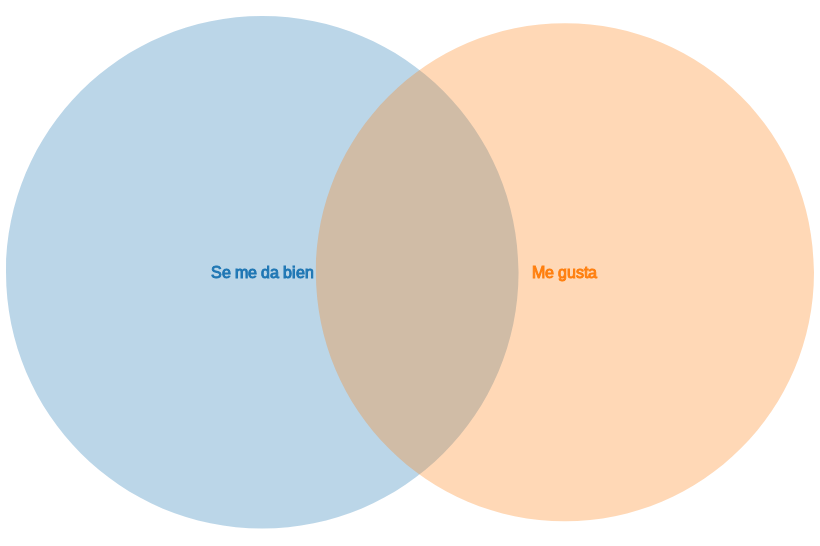
\includegraphics[width=.9\linewidth]{venn-diagram.png}
\end{center}

\subsection{Características personales deseables}
\label{sec:org000000f}
\begin{itemize}
\item Disposición al autoaprendizaje
\item Organización del trabajo
\item Habilidades interpersonales
\item Habilidades comunicativas
\item Matemáticas, especialmente en el desarrollo de aplicaciones
\item Inglés
\end{itemize}


\subsection{Esto no es informática}
\label{sec:org0000012}


\subsection{Cómo saber si me gusta}
\label{sec:org0000015}
\begin{itemize}
\item Programación: \href{https://scratch.mit.edu/}{Scratch} << \href{https://codecombat.com/}{Code Combat} << \href{https://www.aceptaelreto.com/}{Acepta el reto}
\item Bases de datos: \href{https://sqlpd.com/}{SQL Police Department} << \href{https://mystery.knightlab.com/}{SQL Murder Mystery}
\item Sistemas: \href{http://web.mit.edu/mprat/Public/web/Terminus/Web/main.html}{Terminus game} << \href{https://ubuntu.com/download}{Instalar linux}
\item Sistemas y redes: \href{https://overthewire.org/wargames/bandit/bandit0.html}{Bandit}
\end{itemize}
\end{document}
